\documentclass[11pt, titlepage]{article}
\usepackage[utf8]{inputenc}
\usepackage{amssymb}
\usepackage{amsmath}
\usepackage{amsfonts}
\usepackage{indentfirst} % Indent paragraph
\usepackage[norule,bottom]{footmisc} % Footing options
%\usepackage[justification=centering,textfont={sc},labelfont={rm}]{caption}

% Page settings
\usepackage[left=1.5in, right=1.5in, top=1in, bottom=1in]{geometry}
\usepackage{setspace}
\onehalfspacing
%\doublespacing  % \singlespacing 

% Font
\usepackage{lmodern}
	% times, palatino, lmodern, tgtermes
	% bookman, charter, tgschola, pslatex
%\renewcommand{\familydefault}{tgbonum}

% Tools
\usepackage{beamerarticle} % Not sure
\usepackage{todonotes} % Todos
\usepackage{appendix} % Appendix
\usepackage{array,booktabs,longtable,rotating} % Tables
\usepackage{siunitx} % Align decimal points within tables
%\usepackage{lineno}+ %\linenumbers

% Sections, captions, etc.
\usepackage{sectsty} % Section styles
\sectionfont{\centering\scshape} % \normalfont
\subsectionfont{\centering\scshape}
\usepackage{titlesec}
\titlelabel{\thetitle.\quad}
%\titleformat{\subsubsection}[runin]{\em}{\thesubsubsection}{1em}{}
\titleformat{\subsubsection}[runin]{\em}{}{1em}{}


% Links
\usepackage{hyperref}
\hypersetup{%
  draft
%  colorlinks=false,% hyperlinks will be black
%  linkbordercolor=false,% hyperlink borders will be red
%  pdfborderstyle={/S/U/W 1}% border style will be underline of width 1pt
}

% Position tables {here, top, bottom, page}
\makeatletter
\def\fps@table{htbp}
\makeatother

%% ... at the end of paper
\usepackage{endfloat} % if needed, check package "float"

% Create new minipage environment for notes 
% at the bottom of tables or figures
\newenvironment{tablenotes}[1][Note:]{
  \vskip 1.8ex
  \begin{minipage}{\textwidth}\itshape\footnotesize{#1}
} {\end{minipage}}


% Graphics
\usepackage{graphicx,grffile}
\makeatletter
\def\maxwidth{\ifdim\Gin@nat@width>\linewidth\linewidth\else\Gin@nat@width\fi}
\def\maxheight{\ifdim\Gin@nat@height>\textheight\textheight\else\Gin@nat@height\fi}
\makeatother
% Scale images if necessary, so that they will not overflow the page
% margins by default, and it is still possible to overwrite the defaults
% using explicit options in \includegraphics[width, height, ...]{}
\setkeys{Gin}{width=\maxwidth,height=\maxheight,keepaspectratio}
% set default figure placement to htbp
\makeatletter
\def\fps@figure{htbp}
\makeatother

\usepackage{natbib}% plainnat, abbrvnat
\bibliographystyle{plainnat}
\setcitestyle{authoryear,open={(},close={)}}
%\bibliographystyle{aer}


\setlength{\emergencystretch}{3em}  % prevent overfull lines
\providecommand{\tightlist}{%
  \setlength{\itemsep}{0pt}\setlength{\parskip}{0pt}}



\title{Appendix for the paper ``Incentives for Public Goods Inside
Organizations: Field Experimental Evidence''}
\author{Andrea Blasco \and Olivia S. Jung \and Karim R. Lakhani \and Michael Menietti}
\date{Last updated: 16 March, 2018}

\begin{document}
\maketitle


\clearpage
\tableofcontents
\setcounter{tocdepth}{2}
\clearpage

\section{Extended model with heterogenous
costs}\label{extended-model-with-heterogenous-costs}

Consider the case of two types of agents \(j=1,2\) forming two groups of
equal size \(n_1=n_2=n\). Agents can decide to contribute with a single
proposal or not. When an agent of type \(j\) decides to contribute, then
the expected utility is:

\begin{equation}
  u_1^j = \gamma\hat Y + \delta_j + \sum_{k_j=1}^n \sum_{k_l=0}^n \Pr(Y=k_j+k_l) \frac{R}{k_j+k_l} - c_j.
\end{equation}

When an agent of type \(j\) decides to not contribute, then the utility
is:

\begin{equation}
 u_0^j = \gamma (\hat Y - 1).
\end{equation}

Equating these two conditions for all individuals gives the following
mixed-strategy equilibrium condition:

\begin{equation}
\sum_{k_j=1}^n \sum_{k_l=0}^n \Pr(Y=k_j+k_l) \frac{R}{k_j+k_l} 
  = c_j -\delta_j + \gamma \quad\text{for all}\quad j=1,2.
\end{equation}

To examine differences in equilibrium probabilities \(p_1^*\) and
\(p_2^*\), we use the ratio between the above equilibrium condition for
individuals of type \(j=1\) and the same expression for agents of type
\(j=2\). This gives:

\begin{equation}
\frac{\sum_{k_1=1}^n \sum_{k_2=0}^n \Pr(Y=k_1+k_2) \frac{R}{k_1+k_2}}{\sum_{k_1=0}^n \sum_{k_2=1}^n \Pr(Y=k_1+k_2) \frac{R}{k_1+k_2}} = \frac{c_1 -\delta_1 + \gamma}{c_2 -\delta_2 + \gamma}.
\end{equation}

The left hand side can be rearranged as follows.

\begin{equation}
\frac{\Pr(k_2=0) \sum_{k_1=1}^n\Pr(Y=k_1)\frac{R}{k_1} +  \sigma R}{\Pr(k_1=0) \sum_{k_2=1}^n\Pr(Y=k_2)\frac{R}{k_2} +  \sigma R} 
\end{equation}

where
\(\sigma = \sum_{k_1=1}^n \sum_{k_2=1}^n \Pr(Y=k_1+k_2) \frac{1}{k_1+k_2}\).
Using \(1-p_2=\Pr(k_2=0)\) and \(1-p_1=\Pr(k_1=0)\) together with the
density of the binomial distribution, we obtain the following simpler
expression.

\begin{equation}
\frac{(1-p_2) \frac{(1- (1-p_1)^n)}{n p_1} R +  \sigma R }{(1-p_1) \frac{(1- (1-p_2)^n)}{n p_2} R +  \sigma R}  .
\end{equation}

If \(c_1 - \delta_1 > c_2 - \delta_2\), then the above expression in
equilibrium needs to be larger than one. This inequality can be
expressed as follows:

\begin{equation}
\frac{p_2 (1-p_2)}{(1- (1-p_2)^n)}  > \frac{p_1 (1-p_1)}{(1- (1-p_1)^n)}.
\end{equation}

Hence, the inequality is satisfied only if \(p_2\) is greater than
\(p_1\). This proves the statement reported in the paper that if
individuals have heterogeneous costs, then the probability of
contributing a proposal to improve the organization is higher for agents
with lower costs.

\section{Solicitation emails and website of the
contest}\label{solicitation-emails-and-website-of-the-contest}

We show copy of the solicitation sent via email (Figure
\ref{app: solicitation}) and the graphics automatically matching the
treatment of the employee signing in to the contest's website (Figure
\ref{app: graphics}). Finally, we report the text displayed in the
``Rules of the Competition'' section of the contest's website.

\begin{figure}
\centering
\caption{Solicitation email}
\label{app: solicitation}
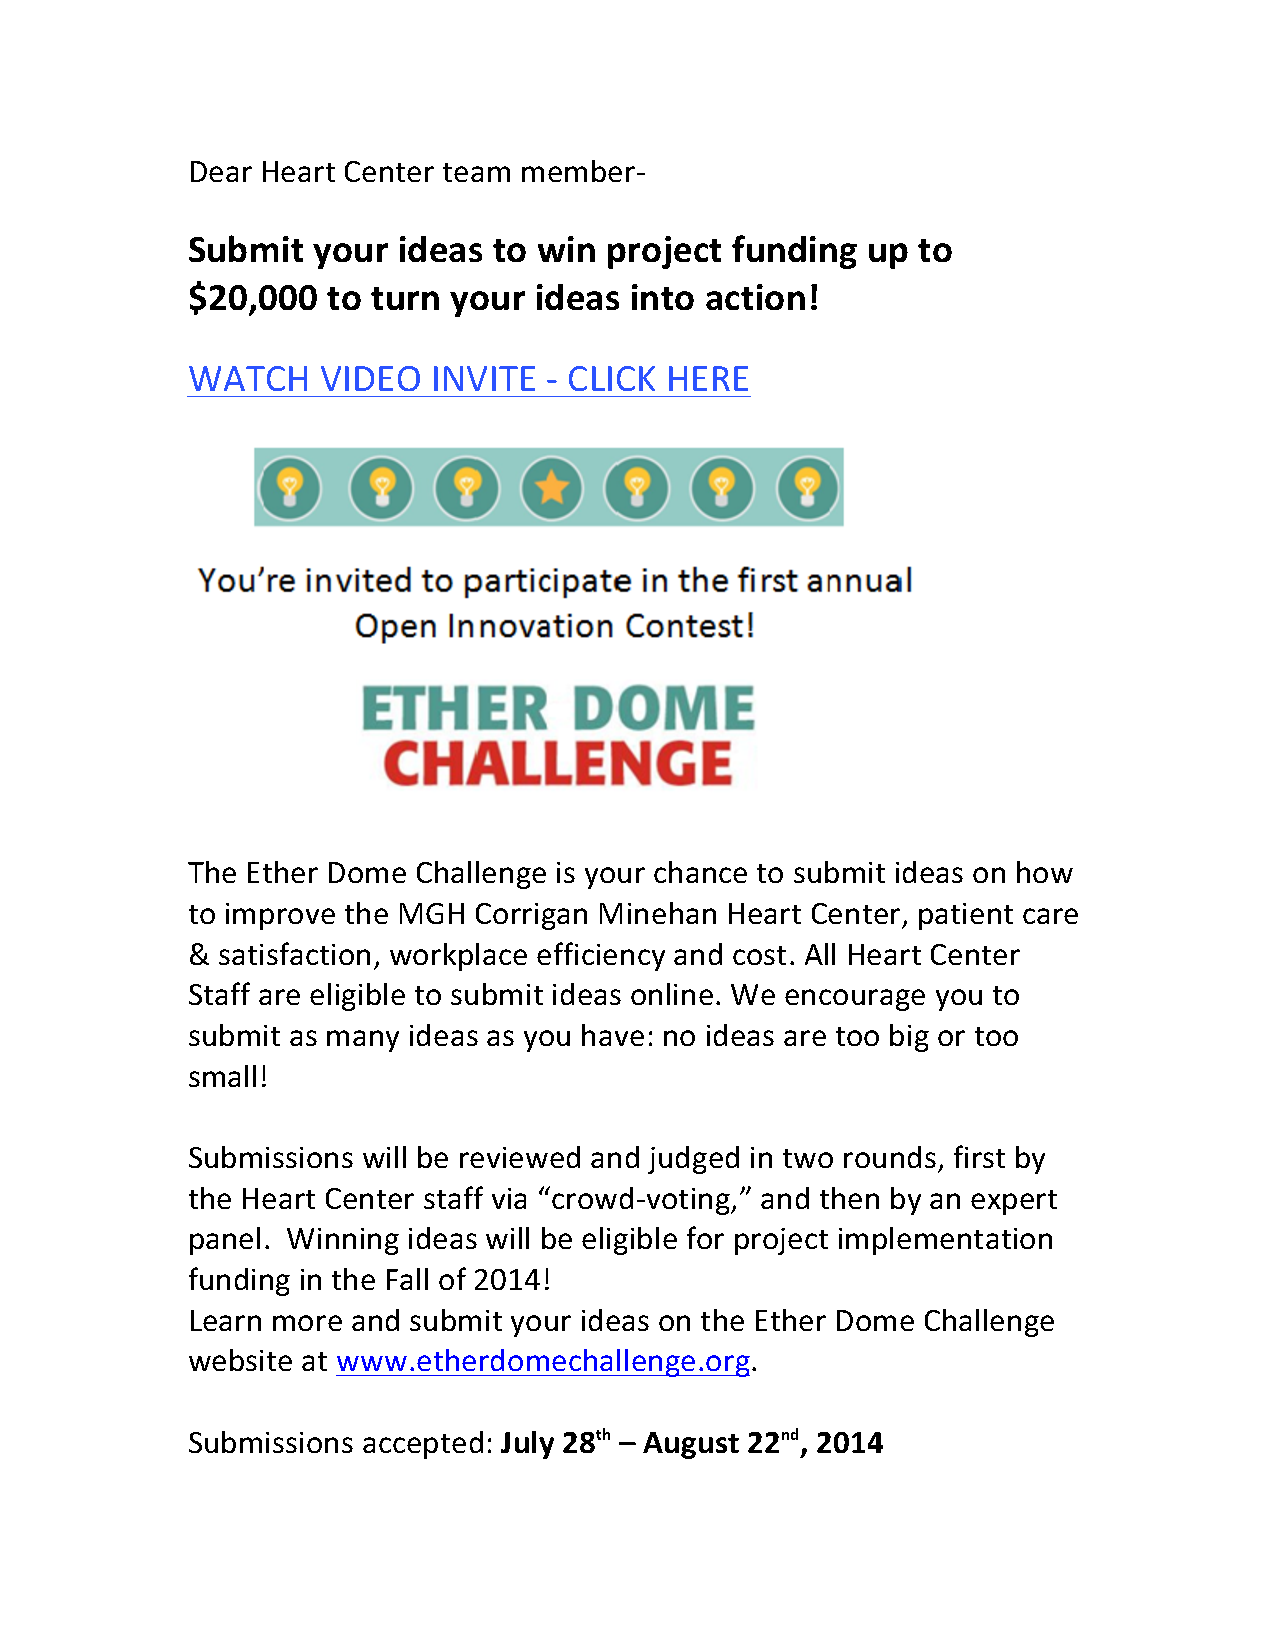
\includegraphics[width=\textwidth]{../figs/img/solicitationEmail.pdf}
\end{figure}

\begin{figure}
\centering
\caption{Treatment matching graphics on the contest's website}
\label{app: graphics}
\begin{tabular}{cc}

\includegraphics[width=2in, height=1.5in]{../figs/img/funding.png} & 

\includegraphics[width=2in, height=1.5in]{../figs/img/money.png} \\
FUND & PRIZE \\

\includegraphics[width=2in, height=1.5in]{../figs/img/patientcare.png} & 

\includegraphics[width=2in, height=1.5in]{../figs/img/workplace.png} \\
PCARE & WPLACE
\end{tabular}
\end{figure}

\subsection{Rules of the competition}\label{rules-of-the-competition}

\begin{itemize}
\item
  The Ether Dome Challenge is an ideas competition to improve the Heart
  Center workplace, patient care, patient satisfaction, workplace
  efficiency and cost.
\item
  If you've noticed something about patient experience, employee
  satisfaction, workplace efficiency, or anything that could be
  improved; if you've had an inspiration about a new way to safeguard
  health; or if you simply have a cost-saving idea, then now is the time
  to share your idea. We would like to encourage all members of the
  Heart Center to participate in this initiative. We encourage you to
  submit as many ideas as you have: no ideas are too big or too small!
  You never know\ldots{} your idea could be the next big thing!
\end{itemize}

\emph{Timeline}

\begin{itemize}
\tightlist
\item
  Ideation Contest Launch
\item
  Idea Submission Closes
\item
  Crowd-Voting on Submitted Ideas
\item
  Top 3 Crowd Voting Winners Announced (winners will receive iPads) \&
  Final Round Idea Selections Announced
\item
  Final Round Idea ``Brainstorming'' Support Sessions \& Team
  Submissions Accepted
\item
  Final Round Submissions Due
\item
  Judging Panel Review of Final Round Submissions
\item
  Ether Dome Challenge Final Award Event - Grant Winners Announced!
\end{itemize}

\emph{Logistics of Idea Submissions}

\begin{itemize}
\tightlist
\item
  All Heart Center Staff (physicians, nurses, administrators, etc.) are
  eligible to submit Ideas.
\item
  Ideas should be submitted electronically via this site. Please click
  the ``Submit Your Ideas'' button at the top of the page, to enter the
  Challenge.
\item
  Submit as many ideas as you'd like!
\end{itemize}

\emph{To promote all kinds of ideas\ldots{} even the zanny ones!}

\begin{itemize}
\tightlist
\item
  All ideas submitted during the challenge will be posted on this
  website to be voted on by all Heart Center staff. The best ideas will
  be awarded a prize. To keep voting fair, ideas will be anonymously
  posted to the voting site. If your idea wins, you will be able to
  choose whether or not you'd like recognition for the idea. To ensure
  everyone feels free to submit all types of creative ideas - no matter
  how disruptive - all ideas will remain anonymous and shared only with
  the Harvard Business School study designers and the MGH Healthcare
  Transformation Lab staff. Individual information/ideas will not be
  shared with your managers/division heads, unless you elect for it to
  be shared publicly after the voting period. De-identified idea
  submissions will be shared with all levels of hospital administration
  deemed appropriate by the Healthcare Transformation Lab staff.
\end{itemize}

\emph{Areas of focus - but don't limit your thinking!}

\begin{itemize}
\tightlist
\item
  Areas of focus for the Ether Dome Challenge include, but are not
  limited to: New models of care delivery; Enhancing the patient
  experience; Improving the MGH workplace, Improving efficiency, quality
  and safety; Lowering the cost of care
\end{itemize}

\bibliography{refs.bib}

\end{document}